\documentclass[a4paper,11pt]{article}
\usepackage{amsmath}
\usepackage{epstopdf}
\usepackage{amsfonts}
\usepackage{graphicx}
\usepackage{algorithm,algorithmic}
\usepackage{url}
\usepackage{color}
\usepackage{tikz}
\usepackage{multirow}
\usepackage{verbatim}
%\usepackage{hyperref}
\usepackage{float}
\usepackage{geometry}
\usepackage{indentfirst}
\usepackage{amssymb}
%\usepackage{circuitikz}
\usepackage{array} 
\usepackage{appendix}
\usepackage{float}
\usepackage{graphicx}
\usepackage{url}
\usepackage[colorlinks,linkcolor=blue,anchorcolor=blue,citecolor=blue]{hyperref} % hyper reference to contents
\usepackage{algorithm,algorithmic}
\usepackage{tikz}
\usepackage{suffix}
\usetikzlibrary{arrows,shapes,snakes}





\usepackage[retainorgcmds]{IEEEtrantools}
\geometry{left=3.17cm,right=3.17cm,top=2.54cm,bottom=2.54cm}
\pagestyle{empty}

\newcommand{\opal}{\textsc{OPAL}}
\newcommand{\opalt}{\textsc{OPAL-t }}
\newcommand{\opalcycl}{\textsc{OPAL-cycl}}
\newcommand{\opalmap}{\textsc{OPAL-map }}
\newcommand{\opalenv}{\textsc{OPAL-envelop}}

\newcommand{\mad}{\textsc{mad }}
\newcommand{\madnine}{\textsc{mad9 }}
\newcommand{\madninep}{\textsc{mad9p }}
\newcommand{\madeight}{\textsc{mad8 }}

\newcommand{\classic}{\textsc{classic }}
\newcommand{\hfifepart}{\textsc{H5Part }}
\newcommand{\hfifefe}{\textsc{H5FED }}

\renewcommand{\epsilon}{\varepsilon} 
\renewcommand{\vec}[1]{{\bf #1}} 
\newcommand{\dt}[1]{\frac{\partial #1}{\partial t}}
\newcommand{\dtt}[1]{\frac{\partial^2 #1}{\partial t^2}}
\newcommand{\dtvec}[1]{\frac{\partial {\mathbf #1}}{\partial t}}
\newcommand{\dttvec}[1]{\frac{\partial^2 {\mathbf #1}}{\partial t^2}}
\newcommand{\rot}{\vec{\nabla} \wedge }
\renewcommand{\div}{\vec{\nabla} \cdot }

\def\vec#1{\mathbf{#1}}
\def\vecg#1{\boldsymbol{#1}}
\def\norm#1{\| #1 \|} 
\def\tr{^{\!\top}}

\def\curl{{\bf curl}\,}
\def\curlp{{\rm curl}_p\,}
\def\div{{\rm div}\,}
\def\grad{\nabla}
\def\gradp{\nabla_p}
\def\dotp#1#2{\langle#1,#2\rangle}
\def\eps{\varepsilon}

\newcommand{\mat}[1]{\ensuremath{\boldsymbol{#1}}}
\newcommand{\vect}[1]{\ensuremath{\mathbf{#1}}}
\newcommand{\iprod}[2]{\ensuremath{\langle#1,#2\rangle}}
\newcommand{\abs}[1]{\ensuremath{|#1|}}

\newcommand{\Nedelec}{N\'{e}d\'{e}lec}

\newcommand{\id}[1]{\structure{#1}}

\newcommand {\Co}{{\mathbb{C}}}
\newcommand {\Int}{{\mathbb{Z}}}
\newcommand {\Nat}{{\mathbb{N}}}
%
%
\newcommand {\Hcurl}{{H(\mathbf{curl};\Omega)}}
\newcommand {\Hocurl}{{H_0(\mathbf{curl};\Omega)}}
\newcommand {\Hdiv}{{H(\mathrm{div};\Omega)}}
\newcommand {\Hodiv}{{H_0(\mathbf{div};\Omega)}}
%
\renewcommand {\Re}{{\rm I \kern-2pt R}}
\newcommand{\vc}[1]{\mbox{\boldmath $#1$}}
\newcommand {\RM}[1]{\mathrm{#1}}




\begin{document}
\begin{center}
{\large Benchmark of \opal's Secondary Emission Model against  an Analytical Model with a Parallel Plate Geometry} \\
Chuan Wang, Andreas Adelmann \\
\today\\
\end{center}
\section{Introduction}
A phenomenological probabilistic secondary emission model developed by Furman and Pivi \cite{SE}, and a model based on Vaughan's secondary emission model \cite{VH, FE} have been implemented in \opal\ \cite{OP}. 
The  aim is to enable comprehensive  multipacting simulation within the \opal\ framework. Here we report on a benchmark effort using the two mentioned models on a simple geometry. 
We first review the various analytical models using a parallel plate configuration, with a sinusoidal electric field. This allows us to predict precisely the electron multiplication criterion for this simple setup and, reproduce the analytical results. Then we have compared the multipacting results from \opal\ simulations with the theoretical model.

\section{Review of Theoretical Models of Multipacting in Parallel Plate Geometry} 
\subsection{Classical theory}
The theory is restricted to the case of the simple plane-parallel model of multipactor with a spatially homogeneous rf electric field in between and directed perpendicular to the plates and varying harmonically in time, i.e., 
\begin{equation}
\vec{E}(\vec{z},t) = -\mathbf{\hat{z}}E_0\sin \omega t=-\mathbf{\hat{z}}\frac{V_0}{d}\sin \omega t.
\end{equation} 

The sketch map of the geometry of the analytical model is shown in figure \ref{fig:sk}. Electrons are assumed to oscillate between two parallel plates separated by a distance $d$. The $x$ and $y$ dimensions of the plates are assumed to be infinite. The impact of an electron with the plates is accompanied by a secondary emission yield, which depends on the energy of the primary electron and material type of the multipactor. 
 
\begin{figure}[H]
\begin{center}
\scalebox{0.7}{
\begin{tikzpicture}
\usetikzlibrary{arrows}
\draw [<->,thick] (0,0.8) node (zaxis) [above] {$\mathbf{z}$}
        |- (0.8,0) node (yaxis) [right] {$\mathbf{y}$};
\draw [->,thick] (0,0) -- (-0.5656,-0.5656) node (xaxis) [above] {$\mathbf{x}$};

\draw (-3.5,-1) -- (2.5,-1);
\draw (2.5,-1) -- (5,3);
\draw (0.5,3) -- (5,3);
\draw (-3.5,-1) -- (0.5,3);
\draw [<-] (-3.5,-1.05) -- (-3.5,-2.1) node (d) [left,below] {$\mathbf{d}$};
\draw [<-] (-3.5,-3.75) -- (-3.5,-2.7);
\draw (-3.5,-3.8) -- (2.5,-3.8);
\draw (2.5,-3.8) -- (4.5,-0.5);
\draw (-0.0,-0.5) -- (4.5,-0.5);
\draw (-3.5,-3.8) -- (0.0,-0.5);


\path[draw=black] (3.3,0.5) circle (2pt);
%\node[above=7pt,left=2pt] (I) at (0.5,0.5) {};
\path[draw=black,thick] (5.5,-1) circle (0.4);
\draw [] (3.3,0.5) arc (90:37:2.9);
\path[draw=black] (3.3,-2.5) circle (2pt);
\draw [] (3.3,-2.5) arc (-90:-34:2.6);
\draw [thick] (5.1,-1) sin (5.3,-0.9) cos (5.5,-1) sin (5.7,-1.1) cos (5.9,-1) sin (5.9,-1);
\node[above=7pt,right=12pt] (I) at (5.5,-1) {$\vec{E}=-\mathbf{\hat{z}}\frac{V_0}{d} \sin \omega t$};
\end{tikzpicture}
}
\end{center}
\caption{The geometry of the analytical model.\label{fig:sk}}
\end{figure}
Assuming electrons are initially generated on the surface of the lower parallel plate, i.e., $z=0$ at $t=t_0$ according to figure \ref{fig:sk}, then equation of motion becomes immediately: 
\begin{equation}
\frac{d^2\vec{z}}{dt^2} = -\frac{e}{m}\vec{E}.\label{vec}
\end{equation}
Considering the geometry, equation \eqref{vec} can be simplified in scalar form (along the $z$ axis):
\begin{equation}
\frac{d^2z}{dt^2} = -\frac{e}{m} E_0\sin\omega t= - \frac{e}{m}\frac{V_0}{d}\sin\omega t \label{scalar}
\end{equation}
with $V_0$ being  the peak voltage amplitude between the parallel plates.

Integrating the equation \eqref{scalar} w.r.t variable $t$, we obtain the velocity and position of the electrons:
\begin{equation}
\frac{dz}{dt} =- \frac{e}{m}\frac{V_0}{d}\frac{1}{\omega}\cos\omega t + C_1,\label{velocity}
\end{equation}
\begin{equation}
z = - \frac{e}{m}\frac{V_0}{d}\frac{1}{\omega^2}\sin\omega t+C_1t+C_2.\label{position}
\end{equation}
We are following \cite{PP}, i.e., substitute the initial condition $\frac{dz}{dt}|_{t=t_0}=v_{0}$, $z|_{t=t_0}=0$ into equation \eqref{velocity} and \eqref{position}, and use normalized variables:  $v_{\omega}=eV_0/m\omega d $, $\lambda=\omega d/v_{\omega}$, $u=v_{0}/v_{\omega}$, $\omega t_0=\varphi_0$. For the constants $C_1$ and $C_2$ we get
\begin{equation}
C_1=(u+\cos\varphi_0)v_{\omega} \text{ ~~~~~~~~and }\label{C1}
\end{equation}
\begin{equation}
C_2=\frac{d}{\lambda}\sin\varphi_0-\frac{d}{\lambda}(u+\cos\varphi_0)\varphi_0.\label{C2}
\end{equation}
Thus, we obtain the scaled velocity and absolute position of electrons before they impact as: 
 \begin{equation}
u_t=u+\cos\varphi_0-\cos\omega t.\label{ve}
\end{equation}
\begin{equation}
z=-\frac{d}{\lambda}\sin\omega t+\frac{d}{\lambda}(u+\cos\varphi_0)\omega t+\frac{d}{\lambda}\sin\varphi_0-\frac{d}{\lambda}(u+\cos\varphi_0)\varphi_0.\label{po}
\end{equation}
If the velocity and time when electron impacts the upper plate are denoted as $v_{impact}$, $t_i$, and let $u_i= \frac{v_{impact}}{v_{\omega}}$, $\omega t_i=\psi_0$, then from equation \eqref{ve} and \eqref{po}, 
\begin{equation}
u_i=u+\cos\varphi_0-\cos\psi_0.\label{vimpact}
\end{equation}
\begin{equation}
d=-\frac{d}{\lambda}\sin\psi_0+\frac{d}{\lambda}(u+\cos\varphi_0)\psi_0+\frac{d}{\lambda}\sin\varphi_0-\frac{d}{\lambda}(u+\cos\varphi_0)\varphi_0.\label{pimpact1}
\end{equation}
Multiplying the $\lambda/d$ on both side of the equation \eqref{pimpact1} and rearrange the terms, we get:
\begin{equation}
\lambda=(\psi_0-\varphi_0)(u+\cos\varphi_0)+\sin\varphi_0-\sin\psi_0.\label{pimpact}
\end{equation}

The secondary electrons will be immediately generated after impaction, and follow equation \eqref{scalar} using the same relations of scaled velocity and scaled impact time, but have different initial conditions. According to \cite{PP}, the initial condition for secondaries are
\begin{equation}
\varphi_1=\psi_0-k_0\pi.\label{ini_imp}
\end{equation}
Here, the integer number $k_0=2n_0-1$ is odd and provides a new initial phase within the same interval $-\pi<\varphi_1<\pi$ as $\varphi_0$, the first initial phase. Then the resonance condition will be \cite{PP}
\begin{equation}
\varphi_1=\varphi_0=\varphi_R\label{res}
\end{equation}
where $\varphi_R$ is the resonance phase, which depends on $\lambda$, $u$ and the order of the resonance mode $n$ as follows:
\begin{equation}
\lambda=\pi(2n-1)(u+\cos\varphi_R)+2\sin\varphi_R.\label{mode}
\end{equation}

There are two important requirements, which limit possible values of the resonant phase. First, the starting phase must not be too negative since in this case the electron would return to the plate of birth due to the retarding action of the rf field. Second, the resonance should be stable, i.e., a small deviation of $\varphi_0$ from the resonant value $\varphi_R$ should result in a smaller deviation of $\varphi_1$. According to reference \cite{PN}, the above two requirements could be translated into an explicit resonant criterion
\begin{equation}
v_1<2v_{\omega}<v_2 \label{vlimit}
\end{equation}
and
\begin{eqnarray}
\text{max}\left \{
\begin{array}{cc}
(2n-1)\pi-(2n-1)\pi v/3-4\sqrt{2v/3}\\[1em]
\displaystyle \frac{((2n-1)\pi)^2-4}{((2n-1)\pi)^2+4}\left \{\sqrt{((2n-1)\pi)^2+4(1-v^2)}+(2n-1)\pi v )\right \}
\end{array}
\right \}\nonumber
\\[1em]
<\lambda<\sqrt{((2n-1)\pi)^2+4}.\label{tlimit}
\end{eqnarray}
Here, $v_1$ and $v_2$ are velocities relative to the energies that secondary yield equal to unit. With an additional assumption that $v = 0$, equation \eqref{tlimit} can be simplified as
\begin{equation}
(2n-1)\pi<\lambda<\sqrt{((2n-1)\pi)^2+4}.\label{tlimit_simple}
\end{equation}
%\begin{figure}[H]
%\begin{center}
%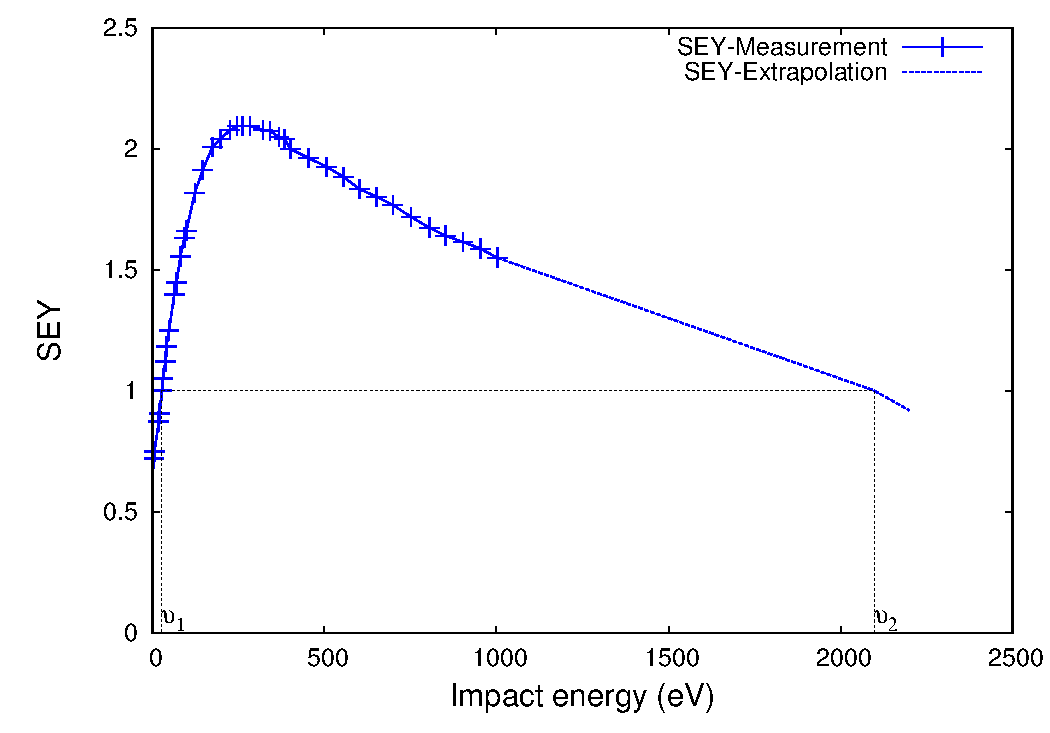
\includegraphics[width=0.6\textwidth]{SEY_curve.pdf}
%\end{center}
%\caption{The SEY curve used in \opal\ simulation.\label{fig:SEY}}
%\end{figure}
Using the resonant criterions \eqref{vlimit} and \eqref{tlimit_simple}, the analytical prediction of resonant zones in Voltage,
$fd$ phase space is shown in figure \ref{fig:bench}.
\begin{figure}[H]
\begin{center}
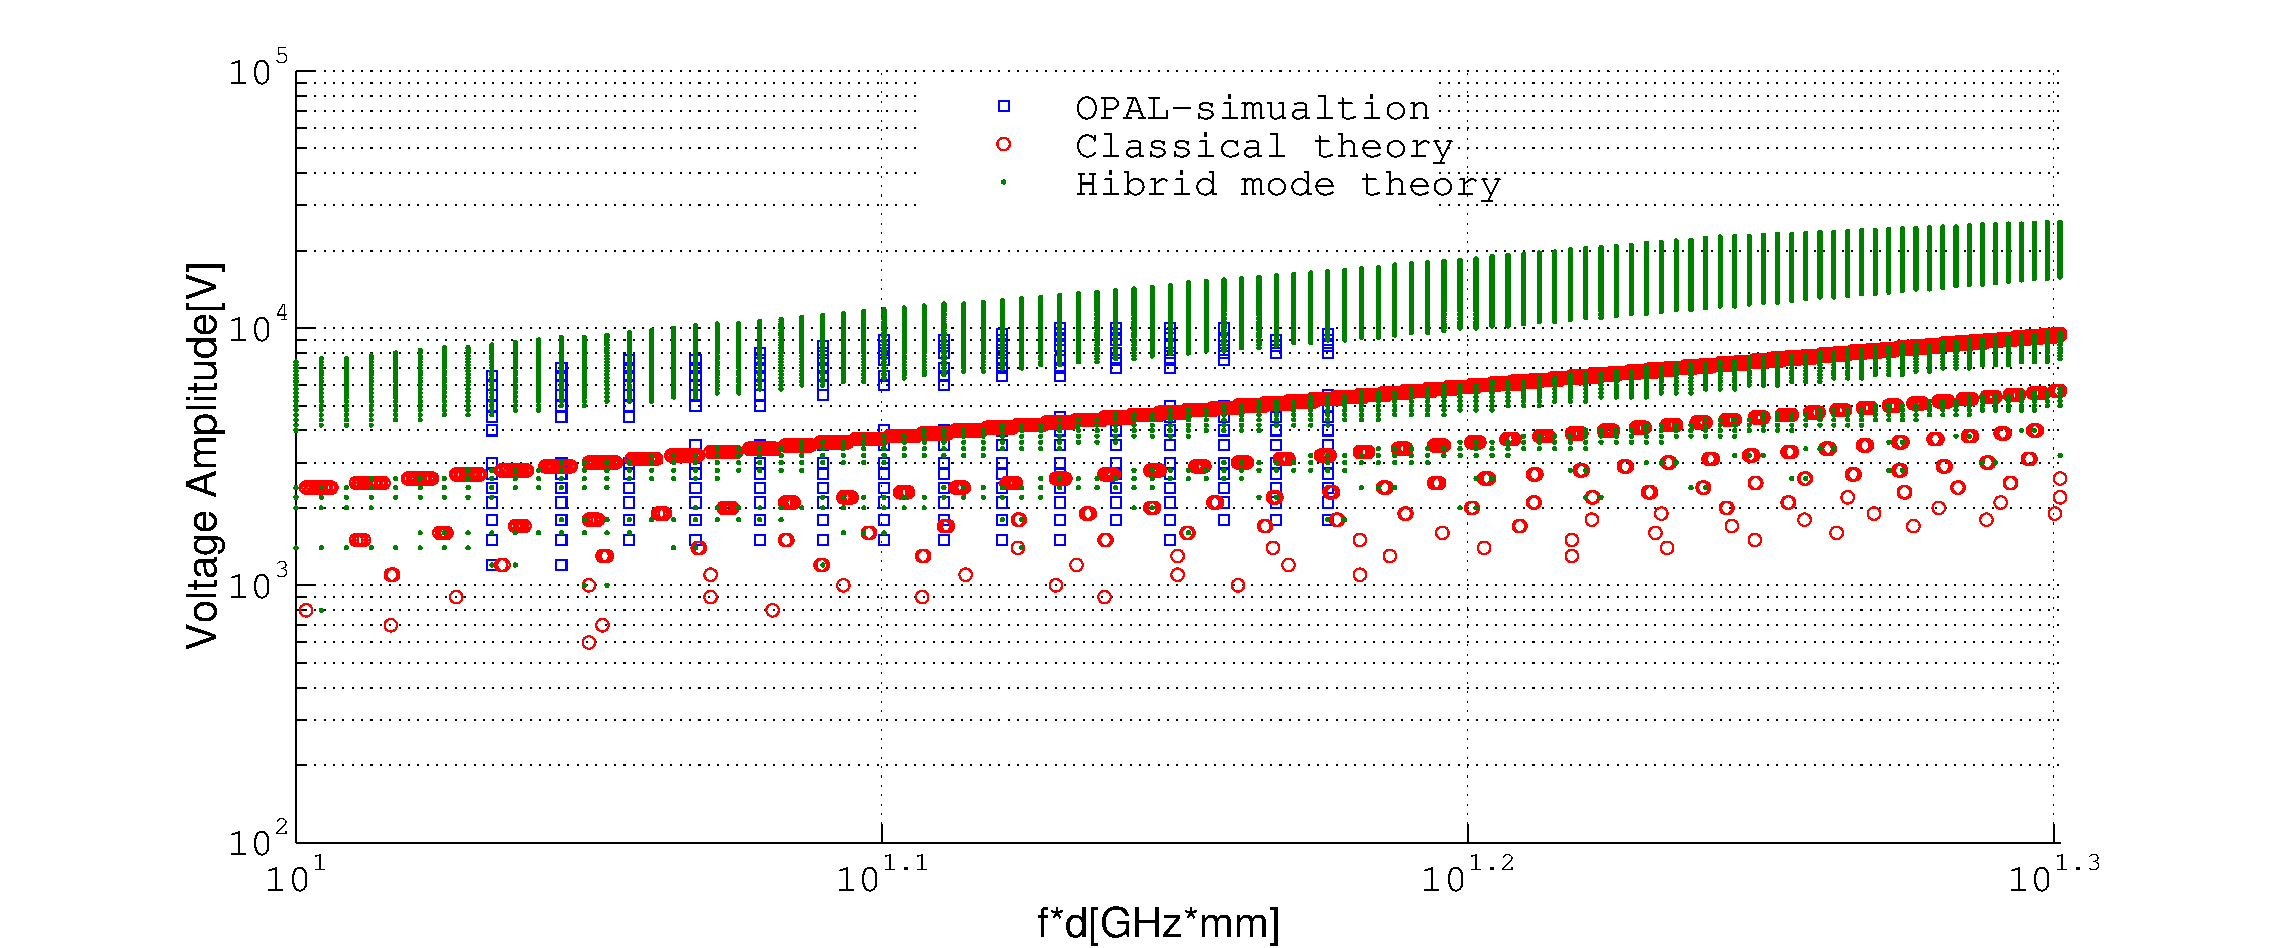
\includegraphics[width=0.8\textwidth]{benchmark2.pdf}
\end{center}
\caption{ The analytical and \opal\ simulation prediction of resonant zone.\label{fig:bench}}
\end{figure}
We have used the following parameter: $d=30mm$, $f=360MHz \sim 500MHz$, $\Delta f=10MHz$, $V_0=600V \sim 10000V$, $\Delta V_0=300V (V_0 \in [600V,3000V])$ and $\Delta V_0=500V (V_0 \in [3000V,10000V])$, with copper's SEY data and Furman-Pivi's secondary emission model in \opal\ simulation and plot the simulation predicted parameter zone where the multiplication occurs also in figure \ref{fig:bench}. The classical theory can not match the simulation even in the first resonant mode and an advanced hybrid mode theory \cite{PP} can only match the simulation in the first resonant mode.
\subsection{Closer to reality: nonstationary statistic theory} 
Although the classic theory clearly reveals the resonant nature of multipactor, however it is far from describing the full picture of the multipactor mechanism and consequently fails to provide reliable breakdown levels \cite{NS}. A nonstationary statistical theory, originated from a stationary statistic theory \cite{ST}, for multipactor introduced by Anza et. al \cite{NS}, gives a more realistic scenario, since it considers the random nature of the electron emission velocity and models both double and single surface impacts, as sketched in figure \ref{fig:ss-ds}.
\begin{figure}[H]
\begin{center}
\scalebox{0.6}{
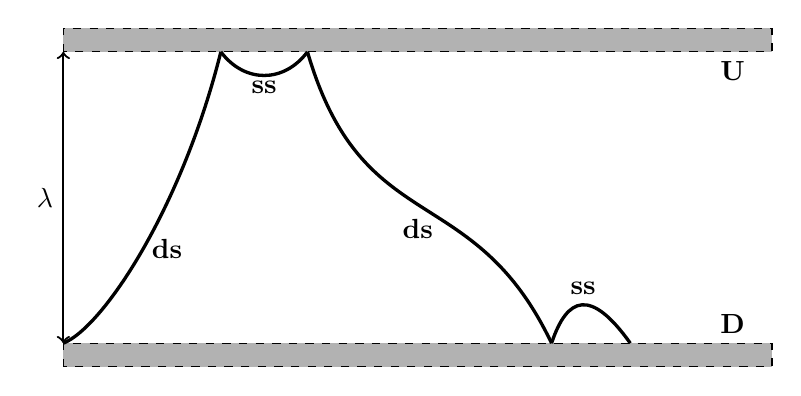
\begin{tikzpicture}
\usetikzlibrary{arrows}
\draw[fill=gray!60,dashed] (-3,0) rectangle (6,0.3);
\draw[fill=gray!60,dashed] (-3,-4) rectangle (6,-3.7);
\draw[very thick] (-3,-3.7) .. controls (-2.5,-3.5) and (-1.5,-2) .. (-1,0);
\draw[very thick] (-1,0) .. controls (-0.7,-0.4) and (-0.2,-0.4) .. (0.1,0);
\draw[very thick] (0.1,0) .. controls (0.8,-2.4) and (2.2,-1.6) .. (3.2,-3.7);
\draw[very thick] (3.2,-3.7) .. controls (3.4,-3.1) and (3.7,-3.0) .. (4.2,-3.7);
\draw (5.5,-3.7) node (d) [above] {$\mathbf{D}$};
\draw (5.5,0) node (u) [below] {$\mathbf{U}$};
\draw (-2.0,-2.5) node (ds1) [right] {$\mathbf{ds}$};
\draw (-0.45,-0.25) node (ss1) [below] {$\mathbf{ss}$};
\draw (1.5,-2) node (ds2) [below] {$\mathbf{ds}$};
\draw (3.6,-3.2) node (ss2) [above] {$\mathbf{ss}$};
%\draw [dashed,thick] (0,0.8) node (zaxis) [above] {$\mathbf{z}$}
%        |- (0.8,0) node (yaxis) [right] {$\mathbf{y}$};
\draw [<-,thick] (-3.,-3.7) -- (-3,-1.85) node (d) [left] {$\mathbf{\lambda}$};
\draw [<-,thick] (-3,0) -- (-3,-1.85);
\end{tikzpicture}
}
\end{center}
\caption{ A full scenario of electron's trajectories between parallel plates, including both double surface (ds) and single surface (ss) impacts. \cite{NS}\label{fig:ss-ds}}
\end{figure}

As described in \cite{NS}, the nonstationary statistical theory also starts from the equation of motion \eqref{vec}, and if we define $\xi=\omega z/v_{\omega}$, equation \eqref{position} can be rewritten by using this new variable as:
\begin{equation}
\xi(\varphi,\varphi_0,u) = (u+\cos \varphi_0)(\varphi-\varphi_0)+\sin \varphi_0 - \sin \varphi.\label{nposition}
\end{equation}
This equation describes the normalized position at phase $\varphi$, with starting phase $\varphi_0$ and initial velocity $u$. Following the definitions in nonstationary theory, each plate will be denoted as $D$ and $U$ for the boundary condition $\xi=0$ (down) and $\xi=\lambda$ (up), respectively. Double and single surface impacts with $D-U$ or $U-D$ and $D-D$ or $U-U$ trajectories will be denoted as $ds$ and $ss$ respectively. Other definitions for the nonstationary theory are given in \cite{NS}, and listed here in Table \ref{my_table} for convenience.
\begin{table}[h]\footnotesize
{\renewcommand{\arraystretch}{1.5}
\renewcommand{\tabcolsep}{0.2cm}}
\caption{Nonstationary theory definitions.}
\centering
  \label{my_table}
  \begin{tabular}{ l  r  }
    \hline
\hline			
    Impact rate (electrons/radian) in plate $U/D$ at phase $\varphi$ & $I_{U/D}(\varphi)$ \\
    Emission rate (electrons/radian) in plate $U/D$ at phase $\varphi$ & $C_{U/D}(\varphi)$ \\
    Number of electrons at time $\varphi$ & $N(\varphi)$ \\
    Probability density that an electron starting at plate $U/D$,\\
    with starting phase $\varphi$, experiences a double/single\\
    surface impact in a transit phase $\tau$ & $G_{ds/ss,U/D}(\tau|\varphi)$\\
    SEY of an electron starting at plate $U/D$, with starting\\
    phase $\varphi$, experiences a double/single surface impact\\
    in a transit phase $\tau$ & $\sigma_{ds/ss,U/D}(\tau|\varphi)$\\

    \hline 
 \hline
  \end{tabular}
 \end{table}

According to Vdovicheva et al. \cite{ST}, the joint probability density $G(\tau|\varphi_0;\lambda)$ is defined as
\begin{equation}
G(\tau|\varphi_0;\lambda)=\left| \frac{\mathrm{d}g(\tau|\varphi_0;\lambda)}{\mathrm{d}\tau} \right| f_u[g(\tau|\varphi_0;\lambda)] \label{gdsdef}
\end{equation}
where $u=g(\tau|\varphi_0;\lambda)$ should be a monotonic function, and is  obtained by working out $u$ from equation \eqref{pimpact} and removing the non-monotonic intervals. The detailed process to obtain $g(\tau|\varphi_0;\lambda)$ and consequently $G(\tau|\varphi_0;\lambda)$ is given in \cite{ST}.

To model the single surface impacts, the nonstationary theory use the joint probability density $G(\tau|\varphi_0;0)$ that the probability density of an electron starting at plate $U/D$, with starting phase $\varphi_0$, experiences single surface impact in a transit phase $\tau$ defined by
\begin{equation}
G(\tau|\varphi_0;0)=\left| \frac{\mathrm{d}g(\tau|\varphi_0;0)}{\mathrm{d}\tau} \right| f_u[g(\tau|\varphi_0;0)] \label{gssdef}
\end{equation}
where the $u=g(\tau|\varphi_0;0)$ is obtained by working out $u$ from equation \eqref{nposition} with an additional condition that $\xi=0$ (and removing the non-monotonic intervals).

As described in the stationary and nonstationary theory, not all the ejection velocity $u$ can be favorable for double or single surface impacts. There exists minimum $g(\tau|\varphi_0;\lambda)$ and maximum $g(\tau|\varphi_0;0)$ \cite{NS,ST} :  
\begin{align*}
 min\{g(\tau|\varphi_0;\lambda)\}=u_{min}\\
 max\{g(\tau|\varphi_0;0)\}=u_{max}
\end{align*}
where $u_{min}=u_{max}$ holds for the same starting phase $\varphi_0$. After setting up the joint probability density $G(\tau|\varphi_0;\lambda)$ and $G(\tau|\varphi_0;0)$, other definitions in Table \ref{my_table} will be given as follows \cite{NS} :
\begin{flalign}
C_U(\varphi)=&\int_0^\varphi C_D(\varphi')G_{ds,D}(\varphi-\varphi'|\varphi')\sigma_{ds,D}(\varphi-\varphi'|\varphi')\mathrm{d}\varphi'\nonumber \\
&+\int_0^\varphi C_U(\varphi')G_{ss,U}(\varphi-\varphi'|\varphi')\sigma_{ss,U}(\varphi-\varphi'|\varphi')\mathrm{d}\varphi'+\Psi_U(\varphi)\label{cudef}
\end{flalign}

\begin{flalign}
C_D(\varphi)=&\int_0^\varphi C_D(\varphi')G_{ss,D}(\varphi-\varphi'|\varphi')\sigma_{ss,D}(\varphi-\varphi'|\varphi')\mathrm{d}\varphi'\nonumber \\
&+\int_0^\varphi C_U(\varphi')G_{ds,U}(\varphi-\varphi'|\varphi')\sigma_{ds,U}(\varphi-\varphi'|\varphi')\mathrm{d}\varphi'+\Psi_D(\varphi)\label{cddef}
\end{flalign}

\begin{flalign}
I_U(\varphi)=&\int_0^\varphi C_D(\varphi')G_{ds,D}(\varphi-\varphi'|\varphi')\mathrm{d}\varphi'\nonumber \\
&+\int_0^\varphi C_U(\varphi')G_{ss,U}(\varphi-\varphi'|\varphi')\mathrm{d}\varphi'\label{iudef}
\end{flalign}

\begin{flalign}
I_D(\varphi)=&\int_0^\varphi C_D(\varphi')G_{ss,D}(\varphi-\varphi'|\varphi')\mathrm{d}\varphi'\nonumber \\
&+\int_0^\varphi C_U(\varphi')G_{ds,U}(\varphi-\varphi'|\varphi')\mathrm{d}\varphi'\label{iddef}
\end{flalign}

\begin{flalign}
N(\varphi)=&\int_0^\varphi \left(C_U(\varphi')+C_D(\varphi')-I_U(\varphi')-I_D(\varphi')\right)\mathrm{d}\varphi'\label{npdef}
\end{flalign}
where $\Psi_U(\varphi)$ and $\Psi_D(\varphi)$ are external electron sources from plate U and plate D, respectively, and the SEY $\sigma_{ds,D}(\varphi-\varphi'|\varphi')$, $\sigma_{ds,U}(\varphi-\varphi'|\varphi')$, $\sigma_{ss,D}(\varphi-\varphi'|\varphi')$, $\sigma_{ss,U}(\varphi-\varphi'|\varphi')$ can be converted to impact velocity related counterparts following the process in reference \cite{ST}.

\section{Benchmarking \opal\ against the Nonstationary Theory}

\subsection{Setting up the benchmark}
The same amount of particles are initialized in both plates (U,D) at the first time step. For the theoretical model, the external source $\Psi_U(\varphi)=\Psi_D(\varphi)=1/2\delta(\varphi)$, where $\delta(\varphi)$ is the Dirac delta function. For consistence between the theoretical model and the \opal\ simulations, we use the SEY curve of copper provided in reference \cite{SE} to benchmark the Furman-Pivi model and the SEY curve of silver given in \cite{NS,FE} in order to benchmark Vaughan's  secondary emission model, (equation \eqref{cudef}, \eqref{cddef}).

The probabilistic model developed  in \cite{SE} maintains the sum of energy of the secondaries which is not  larger than the energy of their impact primary. For simplicity and to be consistent with the theoretical model, we choose the following Maxwellian distribution, the same as in the one in theoretical model \cite{NS} for the initial velocity in \opal
\begin{equation}
f_u=\frac{uv^2_{\omega}}{v^2_t}\exp{\left(-\frac{u^2v^2_{\omega}}{2v^2_t}\right)}\label{maxwellian}
\end{equation}
(instead of using the one in Furman and Pivi's model for the benchmark).

\subsection{Benchmark result}
The first set of parameters we have chosen to perform benchmark is: $f=200$MHz, $V_0=1200$V, $d=30$mm. The material of the multipactor is copper and we calculate the time evolution of the particle number. The results, using  Furman and Pivi's secondary emission model matches the theoretical model very well, as can be seen from figure \ref{fig:results}.   
\begin{figure}[H]
\begin{center}
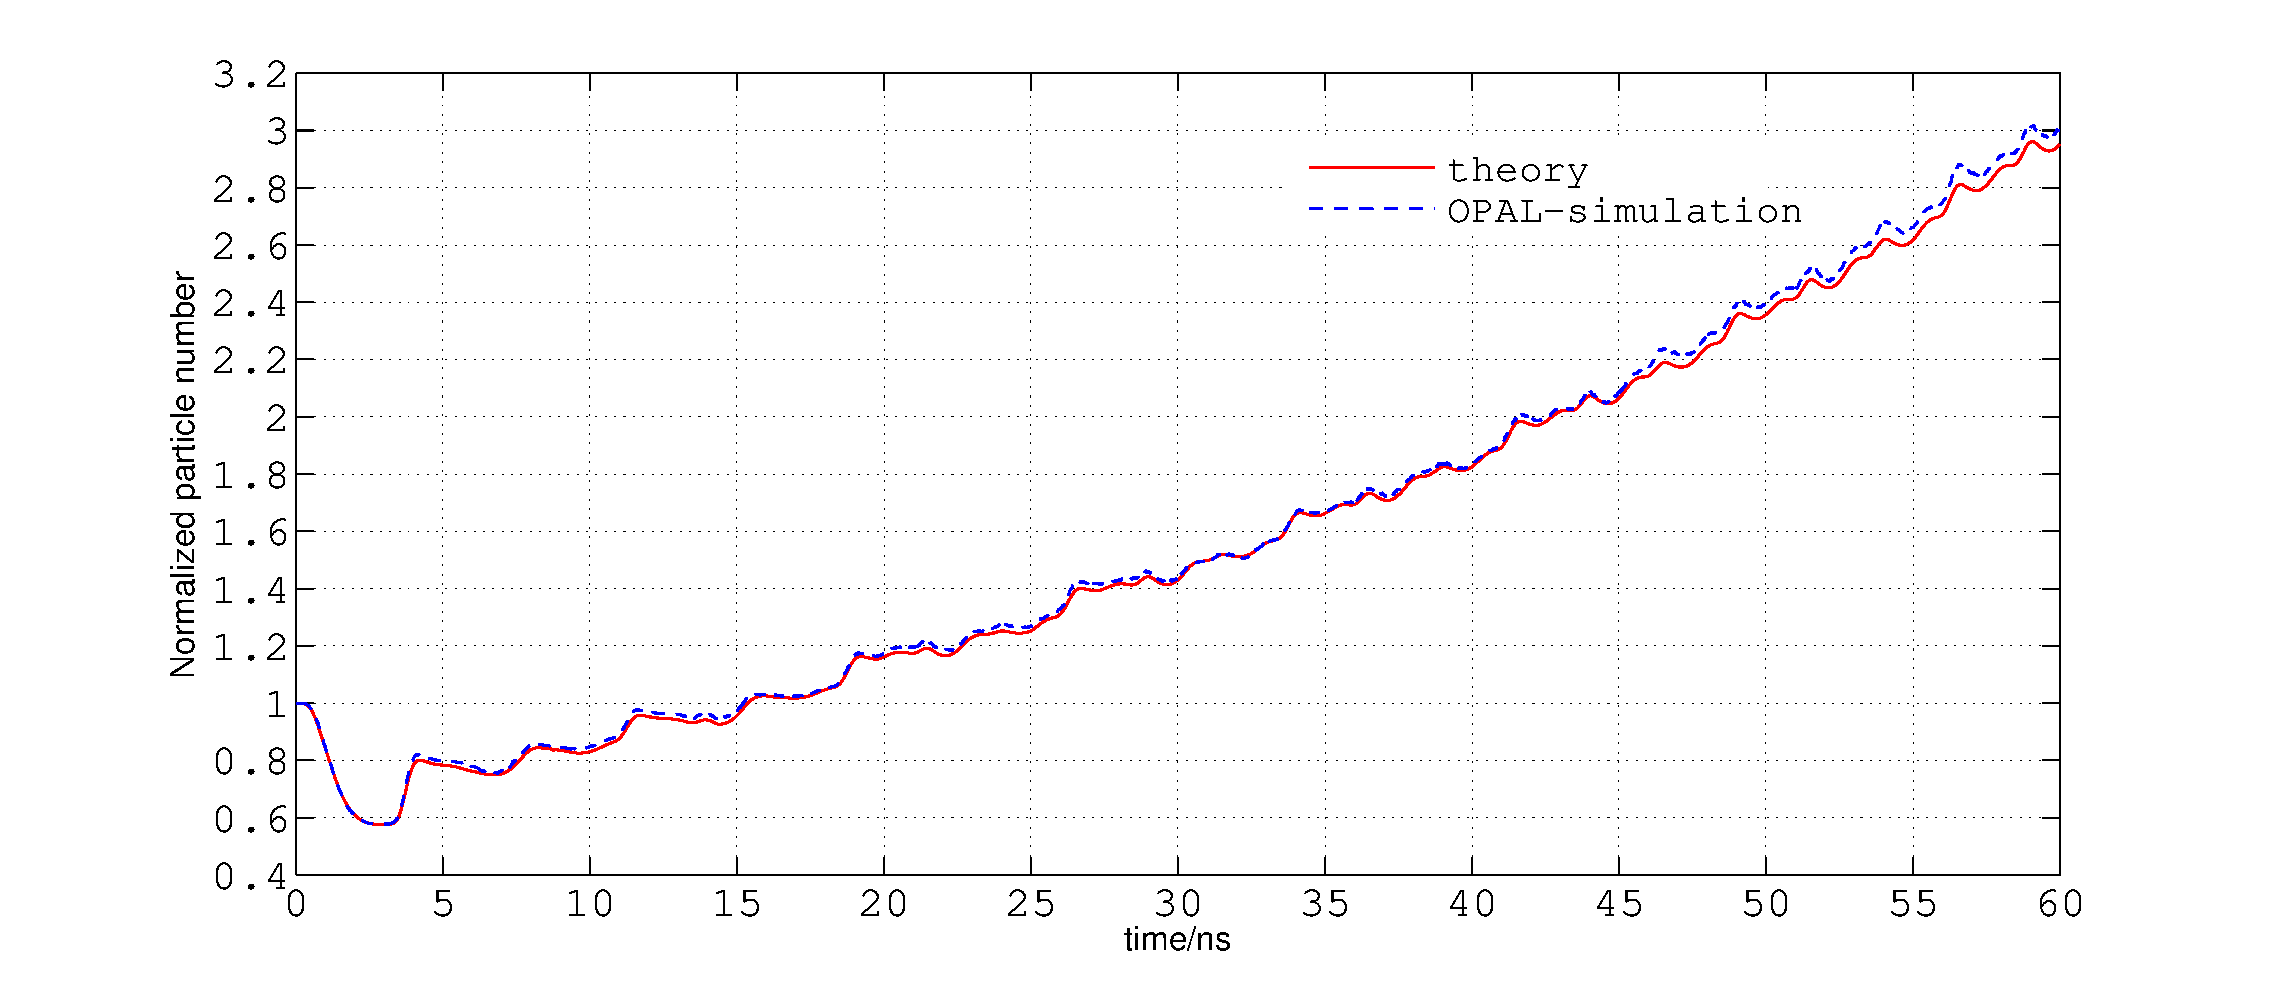
\includegraphics[width=1\textwidth]{match.pdf}
\end{center}
\caption{Time evolution of electron number predicted by theoretical model and \opal\ simulation using Furman and Pivi's secondary emission model at $f=200$MHz, $V_0=1200$V, $d=30$mm.\label{fig:results}}
\end{figure}

The time evolution of electron number under above parameters reaches some equilibrium conditions that the electron population is nether strongly increased nor decreased. The strong multiplication cases have also been observed during benchmark:
\begin{figure}[H]
\begin{center}
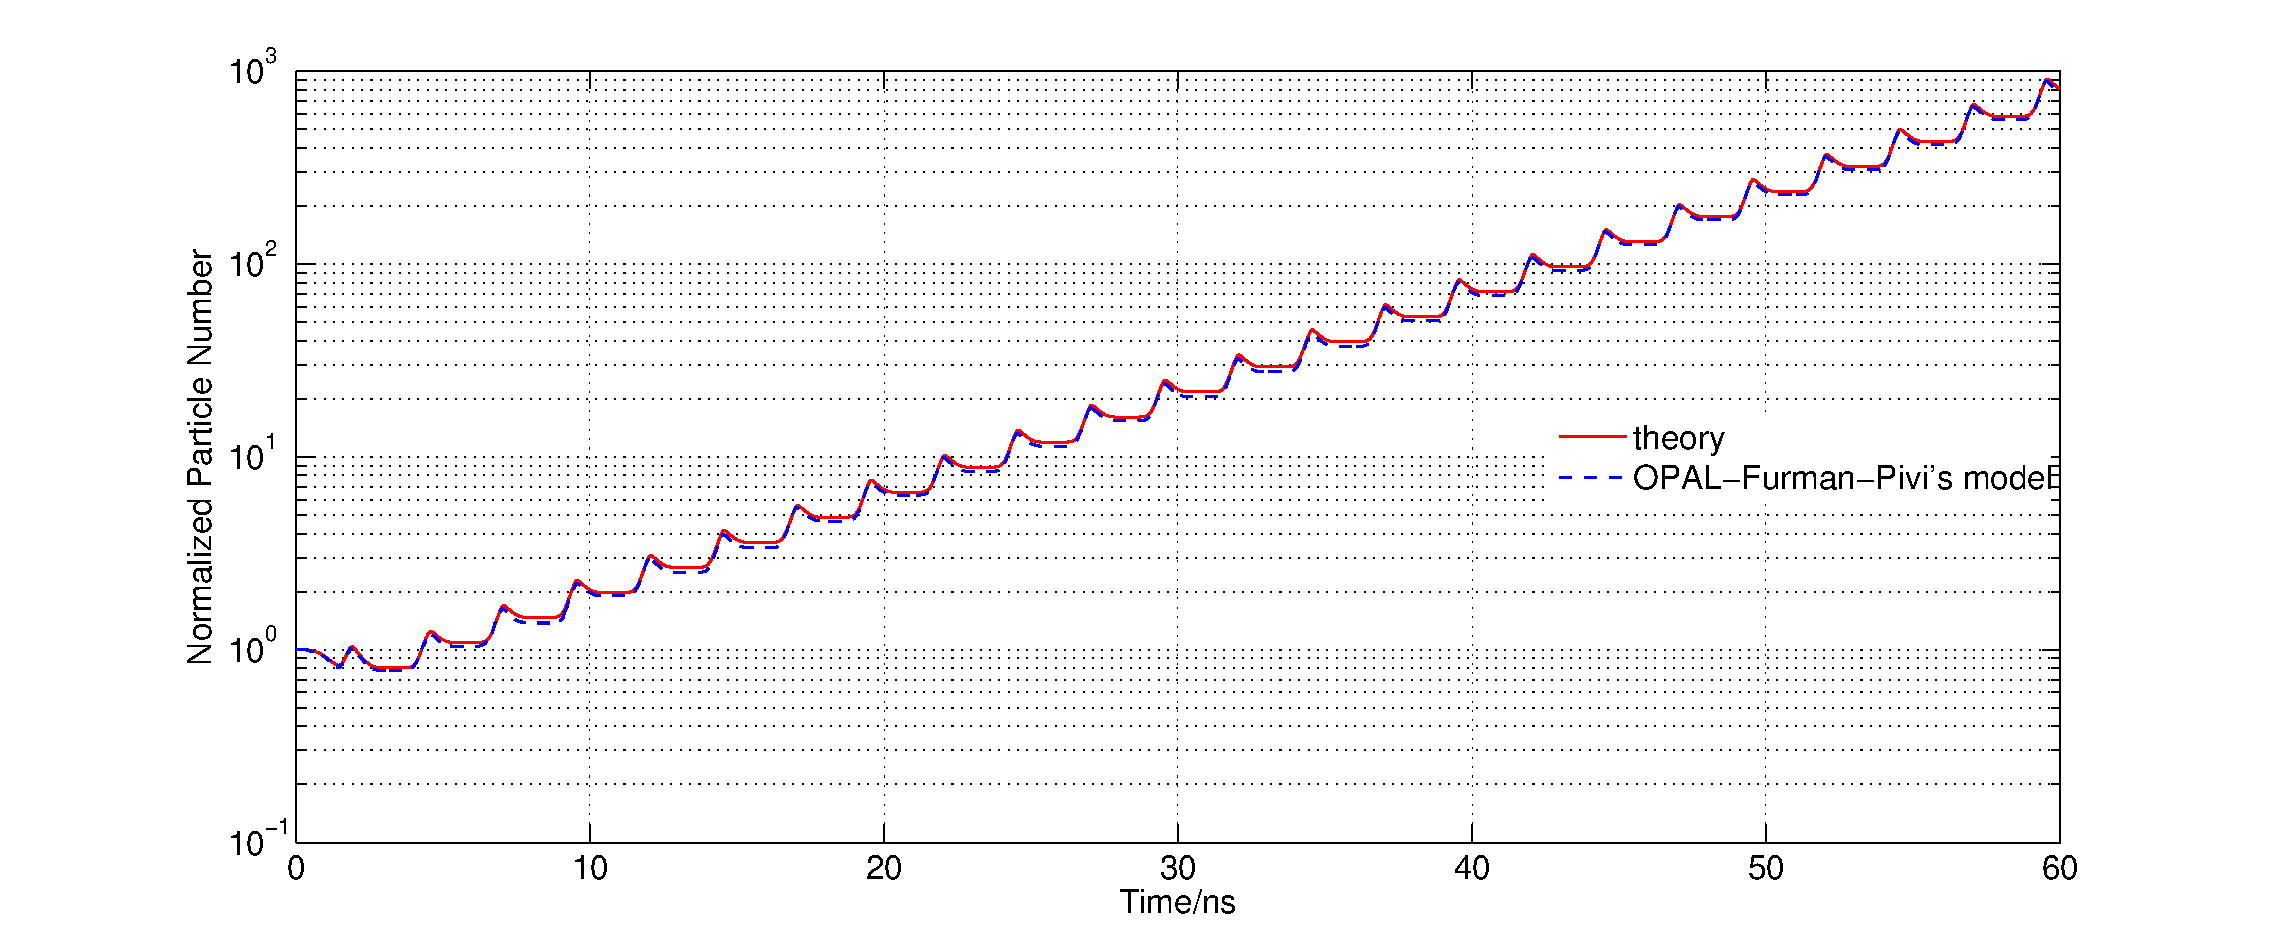
\includegraphics[width=1\textwidth]{copper_multi.pdf}
\end{center}
\caption{Time evolution of electron number at $f=200MHz$, $V_0=120V$, $d=5mm$, using Furman and Pivi's model in simulation and copper's SEY data in theory .\label{fig:multi_copper}}
\end{figure}
\begin{figure}[H]
\begin{center}
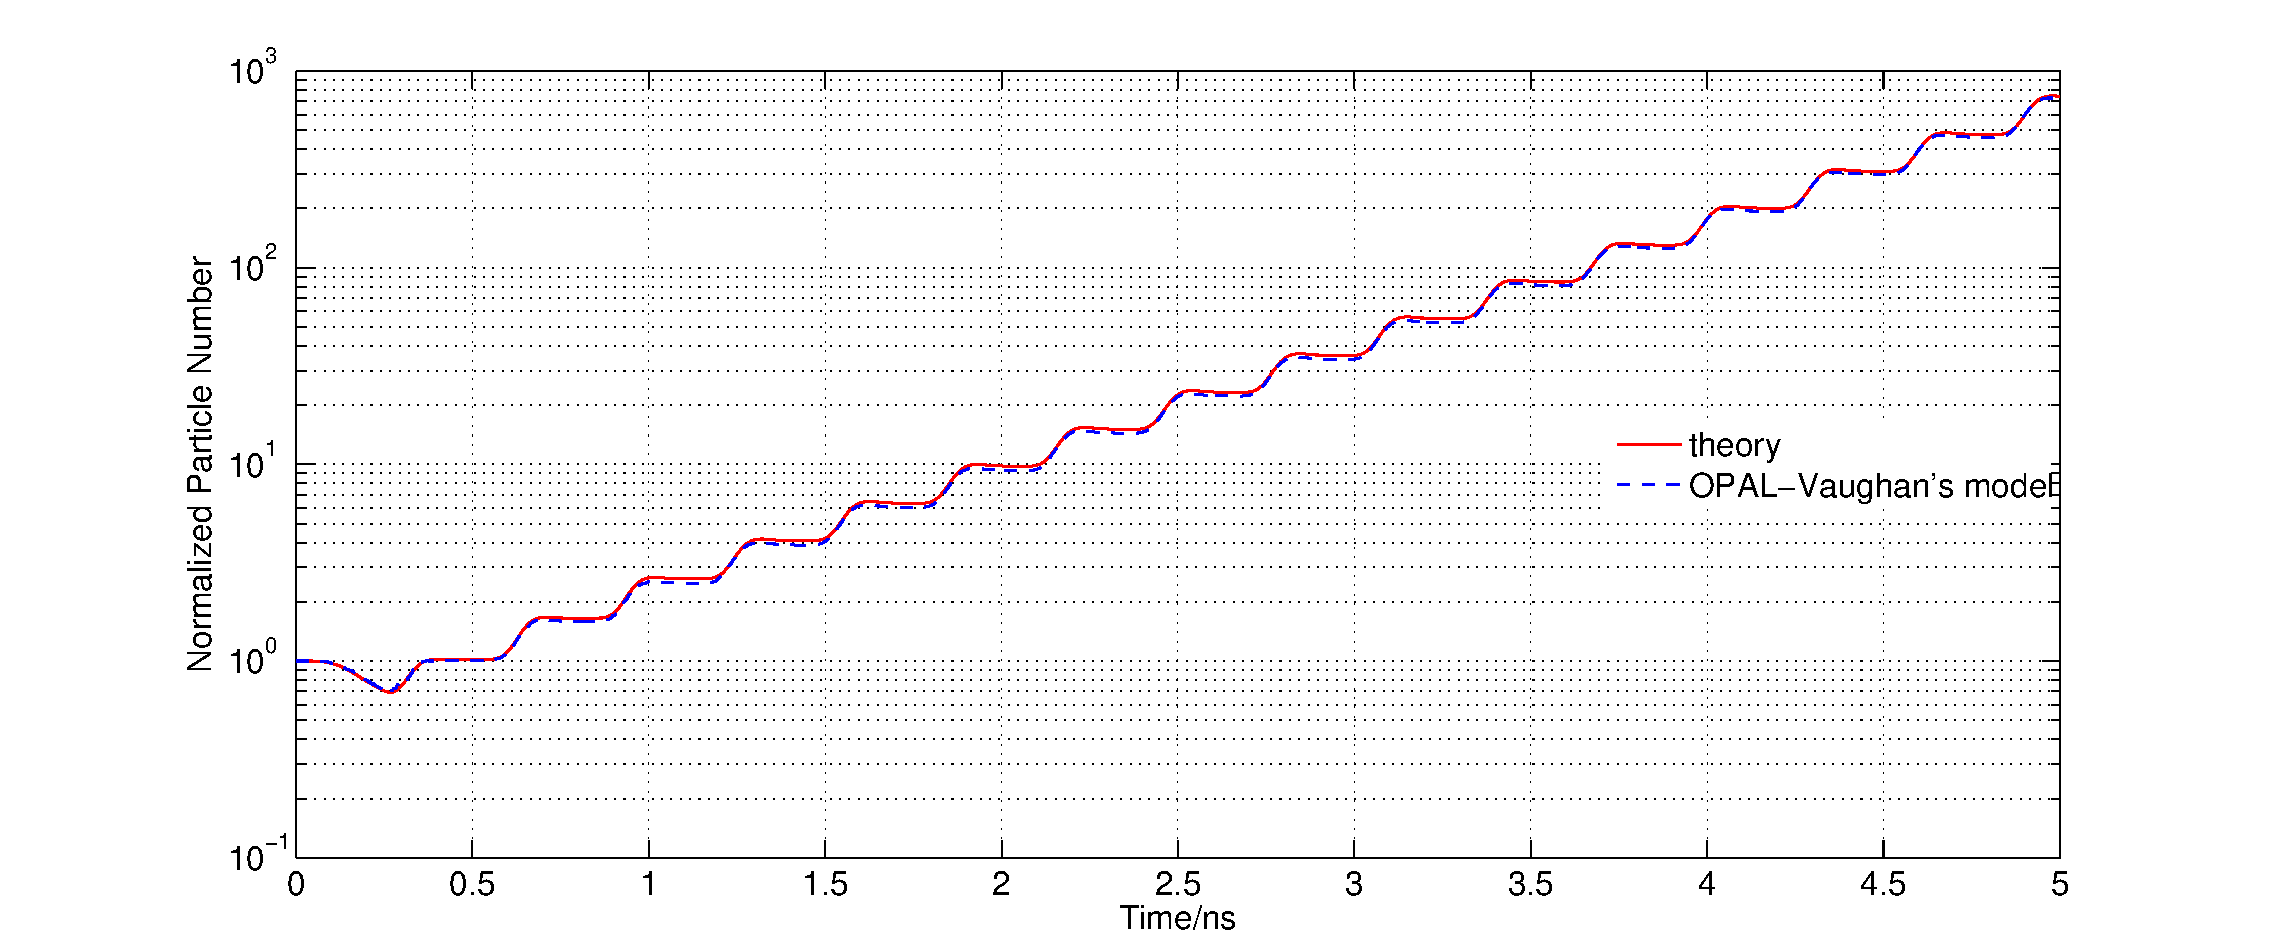
\includegraphics[width=1\textwidth]{silver_multi.pdf}
\end{center}
\caption{Time evolution of electron number at $f=1640MHz$, $V_0=120V$, $d=1mm$, using Vaughan's model in simulation and silver's SEY data in theory.\label{fig:multi_silver}}
\end{figure} 
The deviations of simulation results in figure \ref{fig:multi_copper} and figure \ref{fig:multi_silver} over the theoretical model predicted values are very small and will not increase as integration time increases, as is shown in figure \ref{fig:de}.
\begin{figure}[H]
\begin{center}
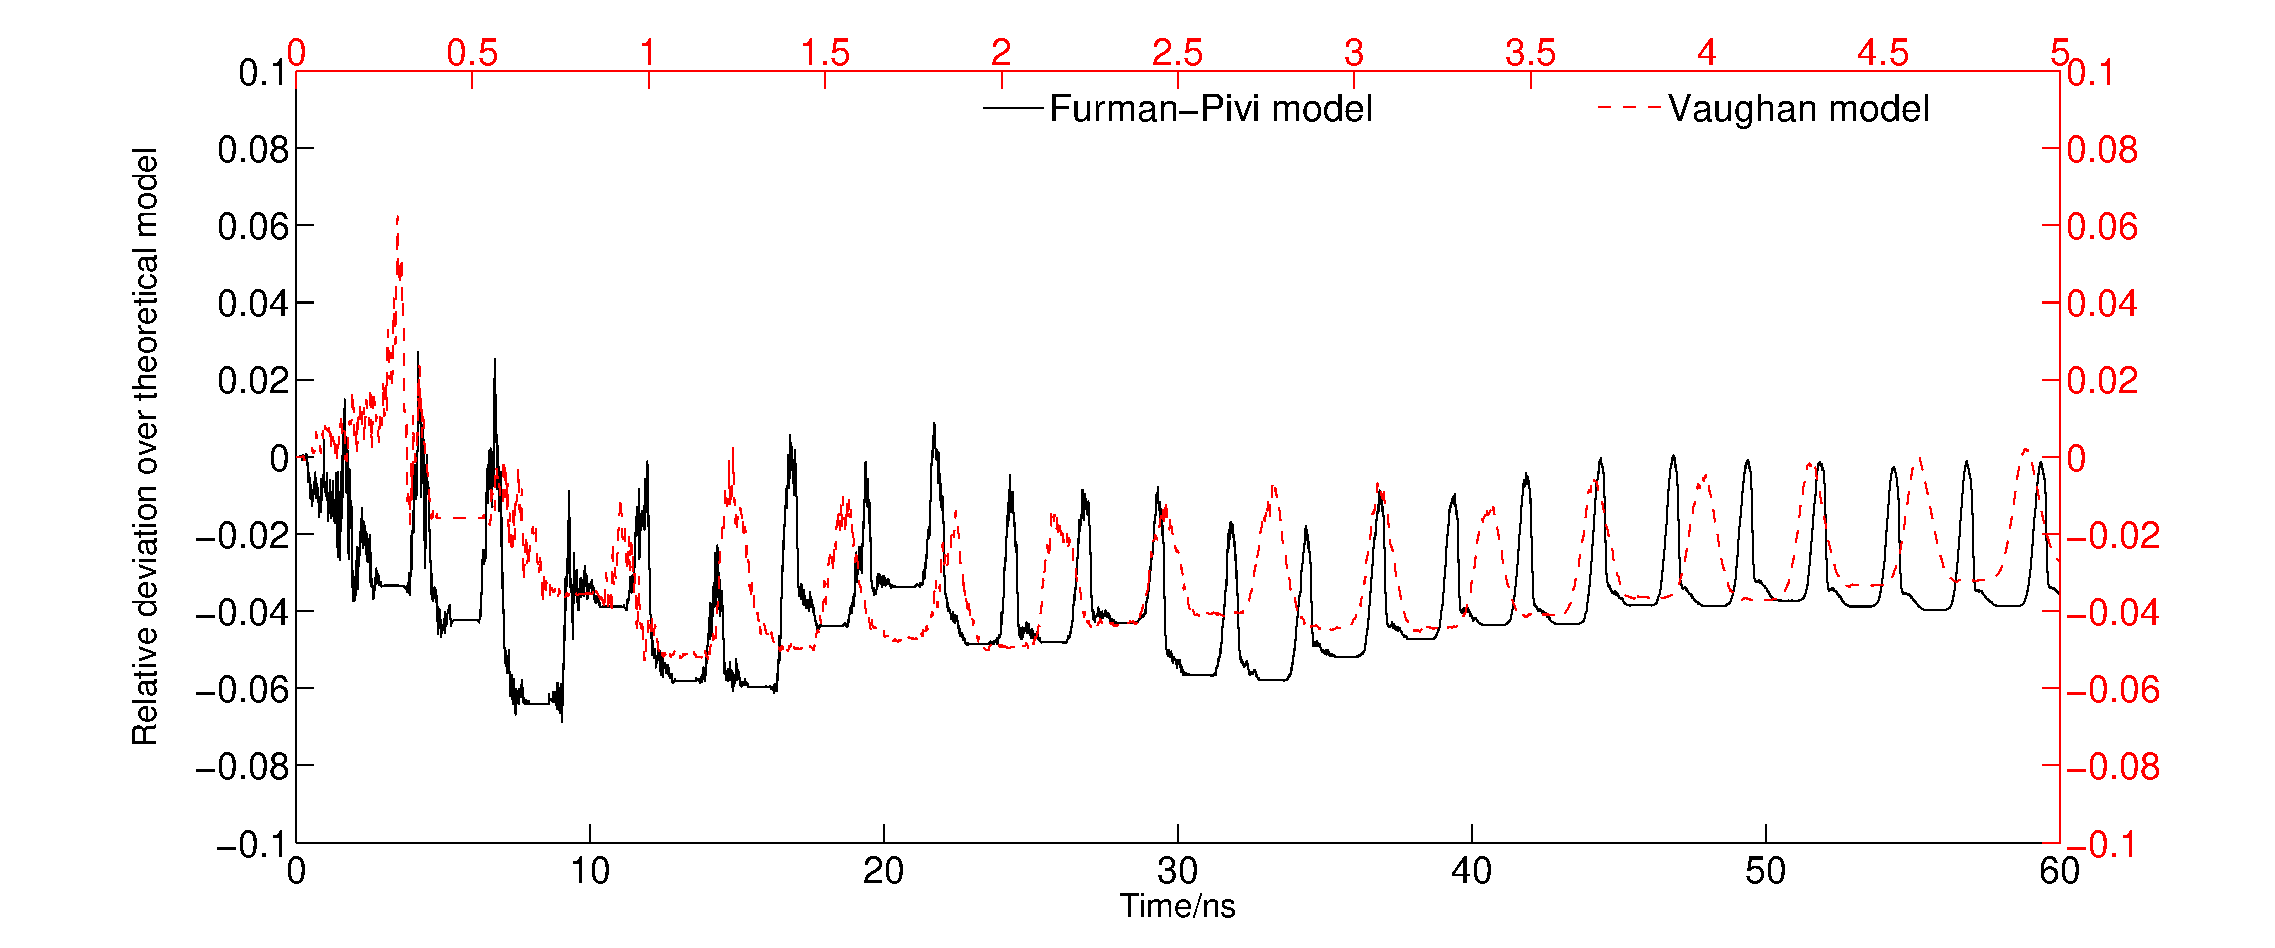
\includegraphics[width=1\textwidth]{models_comp.pdf}
\end{center}
\caption{Time evolution of relative deviations of simulation results using Furman-Pivi's model and Vaughan's model over theoretical model predicted values.\label{fig:de}}
\end{figure}
\begin{appendices}
\section{New Option command in \opal\ for Parallel Plate Benchmark }
To distinguish 3D distributions of initial velocity of secondaries in Furman-Pivi's model and Vaughan's model with the 1 dimensional Maxwellian distribution used in benchmark in a natural way, we add an new boolean variable,  namely ``PPDEBUG" in \opal\ option command. If ``PPDEBUG" is true, then the initial velocity of secondaries will be 1 dimensional Maxwellian distribution in equation \eqref{maxwellian}, otherwise each model will use its own 3D initial velocity distribution. 
\section{Command in \opal\ for Multipacting Simulation}
At present, multipacting module in \opal\ is only implemented in \opalt\ flavor. \opalcycl\ version will be implemented in the near future. As other simulations in \opalt, first the user need to define a transfer line, even if the line contains only one element; then define the distribution of particle bunch; the only difference is to define a boundary geometry contains the surface mesh of the RF structure in which multipacting effects need to be evaluated and define the RF element which attaches the above defined boundary geometry; then as usual, configure the field solver, beam and tracker.       
User can configure the surface physics model in the DISTRIBUTION command, as listed in Table \ref{my_table2} 
\begin{table}[H]\footnotesize
{\renewcommand{\arraystretch}{1.5}
\renewcommand{\tabcolsep}{0.2cm}}
\caption{Command used for Multipacting simulation}
\centering
  \label{my_table2}
  \begin{tabular}{lccc}%{|p{2cm}<{\centering}|p{2cm}<{\centering}|p{2cm}<{\centering}|p{2cm}<{\centering}|p{2cm}<{\centering}|}

\hline\hline %inserts double horizontal lines
Dist. type &Name & Default value & Meaning \\ [0.5ex] % inserts table 
%heading 
\hline % inserts single horizontal line
SE\&SRC &NPDARKCUR & 0.0 & No. of randomly initialized dark current electrons\\ % inserting body of the table
SE\&SRC &INWARDMARGIN & 0.001m & Inward margin of initialized dark current electrons\\
SE &FNA & $1.54\times10^{-6}$ & Empirical constant A for F-N emission model\\
SE &FNB & $6.83\times10^9$ & Empirical constant B for F-N emission model \\
SE &FNY & $3.795\times10^{-5}$ & Constant for image charge effect parameter y(E) \\ [1ex]% [1ex] adds vertical space
 &  &  & ( Use default value of FNY for electrons) \\
SE &FNVYZERO & $0.9632$ & Zero order constant for v(y) function \\
SE &FNVYSECOND & $1.065$ & Second order constant for v(y) function \\ 
SE &FNPHIW & $4.65$ eV & Work function of gun surface material \\ 
SE &FNBETA & $50.0$ & Field enhancement factor $\beta$ for F-N emission \\
SE &FNFIELDTHR & $30.0$ MV/m & Field threshold for F-N emission \\
SE &FNMAXEMI & $20.0$ & Max. No. of electrons emitted from a single triangle \\
SE &VW & $1.0$ m/s & Velocity scalar in Maxwellian Dist. \\
SE &VVTHERMAL & $7.268929821\times10^5$ m/s & Thermal velocity in Maxwellian Dist. \\
SE &SECONDARYFLAG & $0$ & Secondary model type\\
& & &(0:no; 1:Furman-Pivi; $>=$2: Vaughan) \\
SE &NEMISSIONMODE & $\mathbf{true}$ & Emit real No. secondaries or not \\
& & &($\mathbf{true}$:yes; $\mathbf{false}$: const simulation particle number \\
SE &VEZERO& $12.5$ eV & Energy related to $\sigma_0$ in Vaughan's model in eV. \\
SE &VSEYZERO& $0.5$ & $\sigma_0$ in Vaughan's model. \\
SE &VSEYMAX& $2.22$ & $\sigma_{max}$ in Vaughan's model. \\
SE &VEMAX& $165$ & Energy related to $\sigma_{max}$ in Vaughan's model. \\   
SE &VKENERGY& $1.0$ & The roughness of surface for impact energy\\
& & & in Vaughan's model. \\
SE &VKTHETA& $1.0$ & The roughness of surface for impact angle \\
& & &in Vaughan's model. \\  
SE &SURFMATERIAL& $0$ & The material type for Furman-Pivi model \\      
 & & &(0: copper; 1: stainless steel.) \\     
\hline %inserts single line 			
 \hline 
   \end{tabular}
 \end{table}
Here, SE and SRC denote the ``SURFACEEMISSION" and ``SURFACERANDCREATE" type of distribution in \opal.

``SURFACEEMISSION" will hold all the surface physics options available in \opal\, including field emission parameters for Fowler-Nordheim model, parameters for Vaughan's secondary emission model and Furman-Pivi's secondary emission model. 

``SURFACERANDCREATE" will create primary bunch when we simulate the cyclotron cavity and will also be used to create initial electrons in each plates when we do parallel plate benchmark simulation. 

A constant integer named ``MAXPARTSNUM" can be specified in input file to set an upper limit of simulation particle number in simulation.
 
In case of severe multiplication and the number of particles in simulation are too large, an approach using constant number of simulation particles is provided by specifying the ``NEMISSIONMODE" flag to be $\mathbf{false}$ in ``SURFACEEMISSION" distribution. Instead of using random number and Monte-Carlo process to determine the number of secondary emission particles in each impact, this approach maintains the same number of particles in simulation and multiply the current of each impact particle by the factor of SEY. This approach is also a quite accurate representation of secondary emission models, as long as the same energy and emission angle distribution as in the previous real particle emission approach is used in this approach, and can be observed in the following parallel plate benchmarking case.

\begin{figure}[H]
\begin{center}
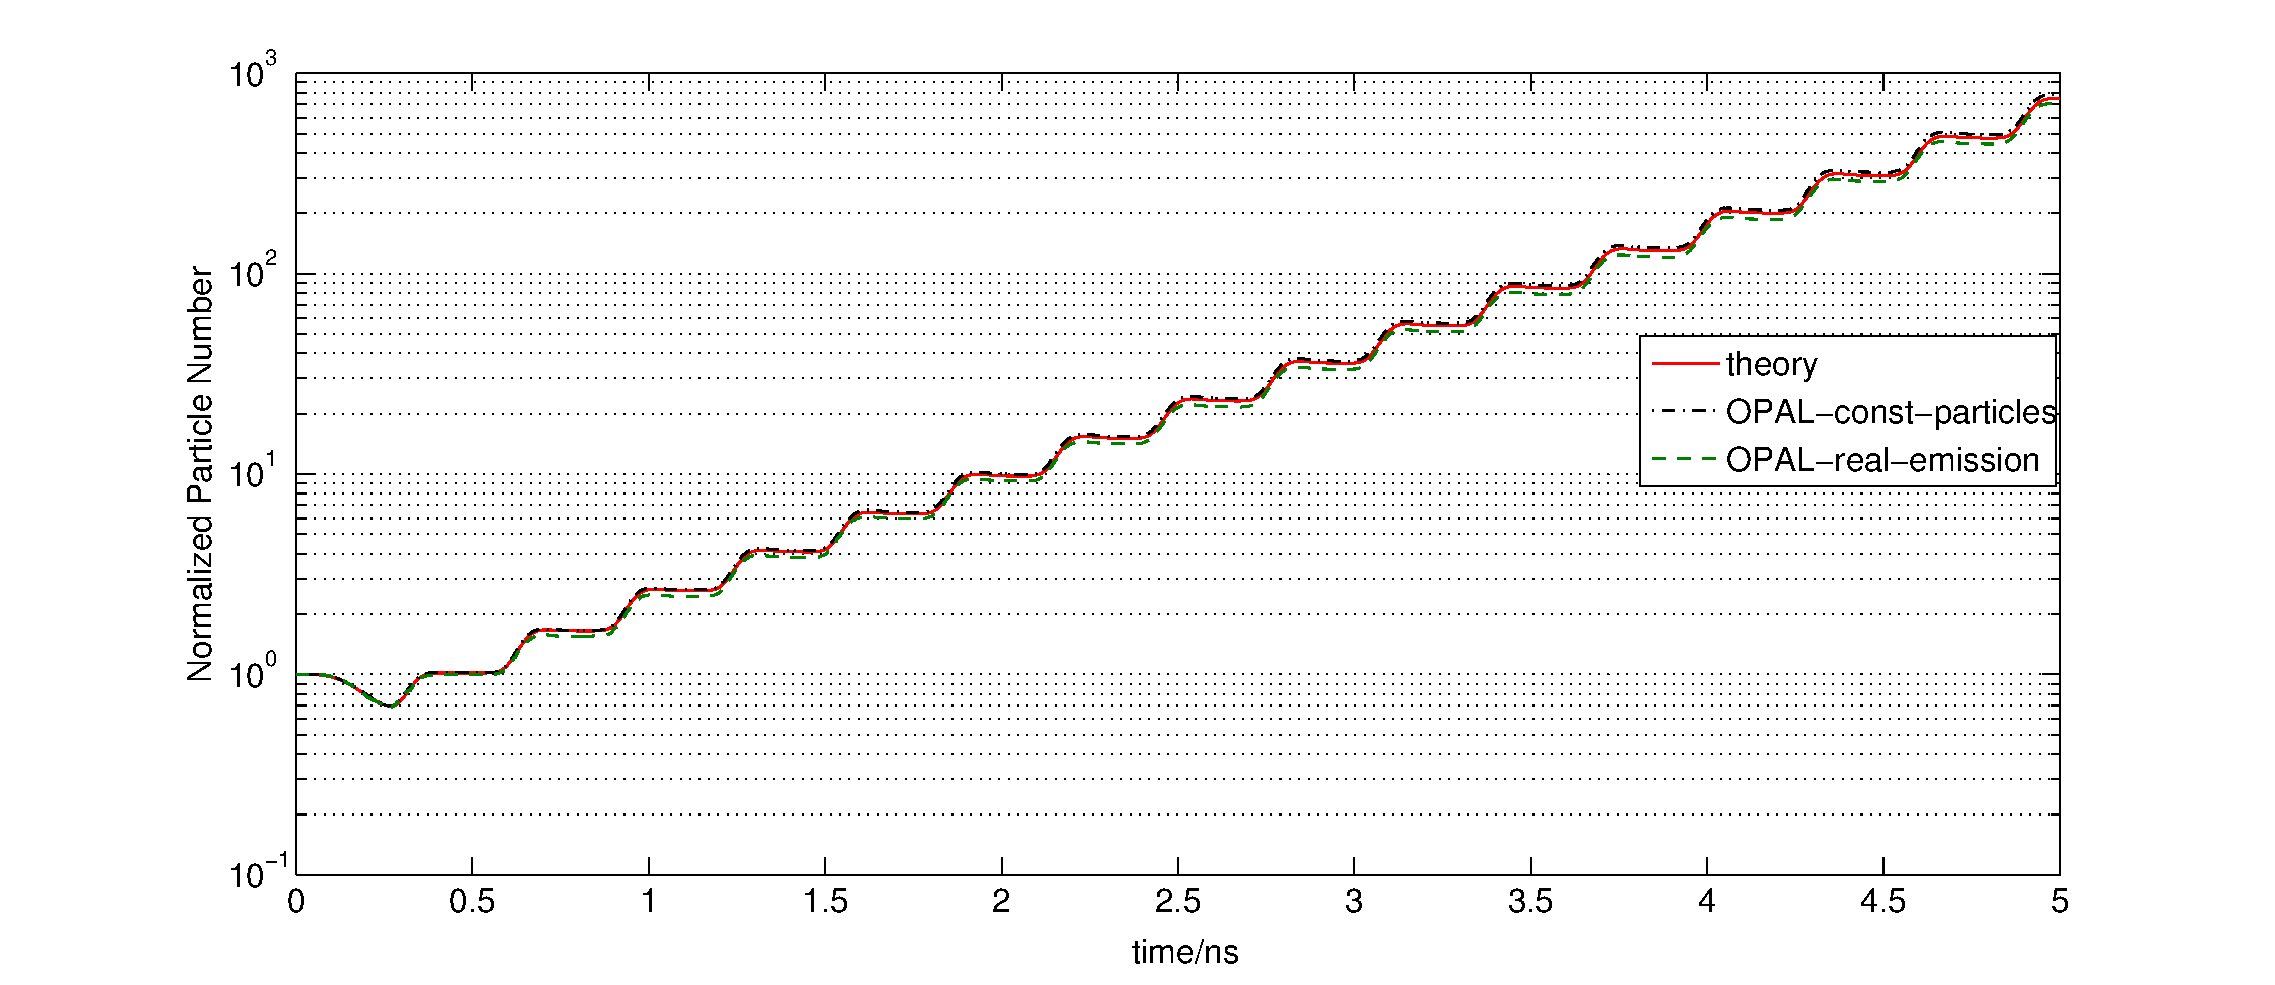
\includegraphics[width=1\textwidth]{const_particle_benchmark.pdf}
\end{center}
\caption{Time evolution of electron number predicted by theoretical model and \opal\ simulation using Vaughan's secondary emission model with both constant simulation particle approach and real emission particle approach at $f=1640$MHz, $V_0=120$V, $d=1$mm.\label{fig:constp}}
\end{figure}

\begin{figure}[H]
\begin{center}
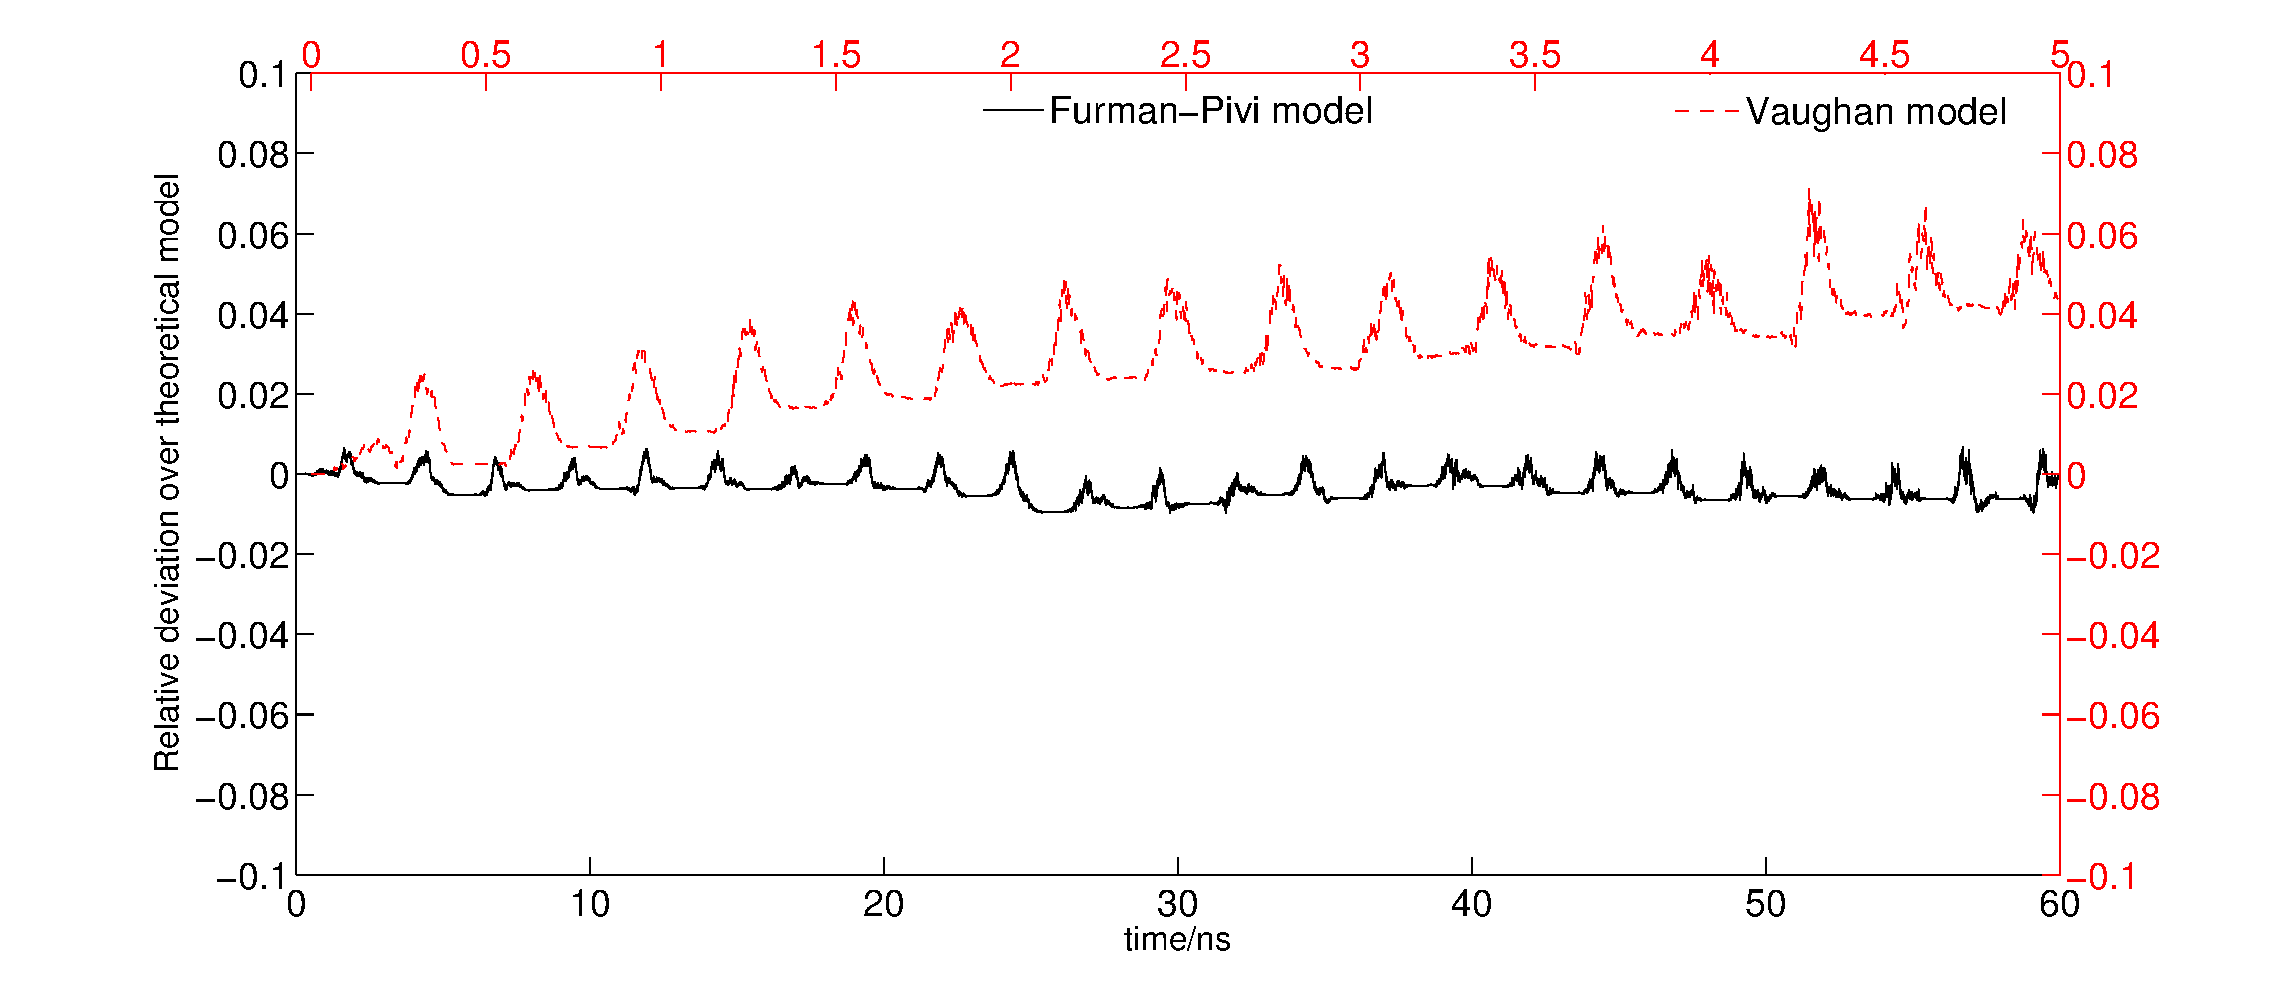
\includegraphics[width=1\textwidth]{models_comp_const_part.pdf}
\end{center}
\caption{Time evolution of relative deviations of simulation results using constant simulation particle approach and both Furman-Pivi's model and Vaughan's model over theoretical model predicted values.\label{fig:de_const}}
\end{figure}
\section{New Elements and Field Maps in \opal\ for Multipacting Simulation}
A new element type ``CYCLOTRONVALLEY", as well as two new field map types ``FM3DH5Block\_nonescale" and ``FM3DMagnetoStaticH5Block" has been implemented in \opal\ to model the multipacting of cyclotron cavities which have already been mounted in the valley of a cyclotron. 

The new element ``CYCLOTRONVALLEY" contains 4 own commands ``FMAPFN", ``DX", ``DY" and ``DZ" which denote the field map file name, the displacement in $\mathbf{x}$, $\mathbf{y}$ and $\mathbf{z}$ direction, respectively and 1 common command ``ELEMEDGE" which denote the start point of the element in $\mathbf{z}$ direction.

New field map ``FM3DH5Block\_nonescale" has almost the same format as the existing type ``FM3DH5Block" except that the former one don't use the $E_{zmax}$ to scale the field map. ``FM3DH5Block\_nonescale" reads field map in ``MV/m", i.e., the same unit as the unit in ``FM3DH5Block".

New field map ``FM3DMagnetoStaticH5Block" also has both ``Efield" and ``Bfield" data sets, however, the electric field parts are zero. This could maintain the same pattern of ``apply" method in ``CYCLOTRONVALLEY" element as in other elements in \opal. The ``Bfield" data should be in ``Gauss", and the ``FM3DMagnetoStaticH5Block" will convert the ``Bfield" data into ``Tesla". The field map will vary first in $\mathbf{x}$, then in $\mathbf{y}$ and finally in $\mathbf{z}$ direction.

The following are example fields stored in ``FM3DH5Block\_nonescale" and ``FM3D\-MagnetoStaticH5Block" formats.

\begin{figure}[H]
\begin{center}
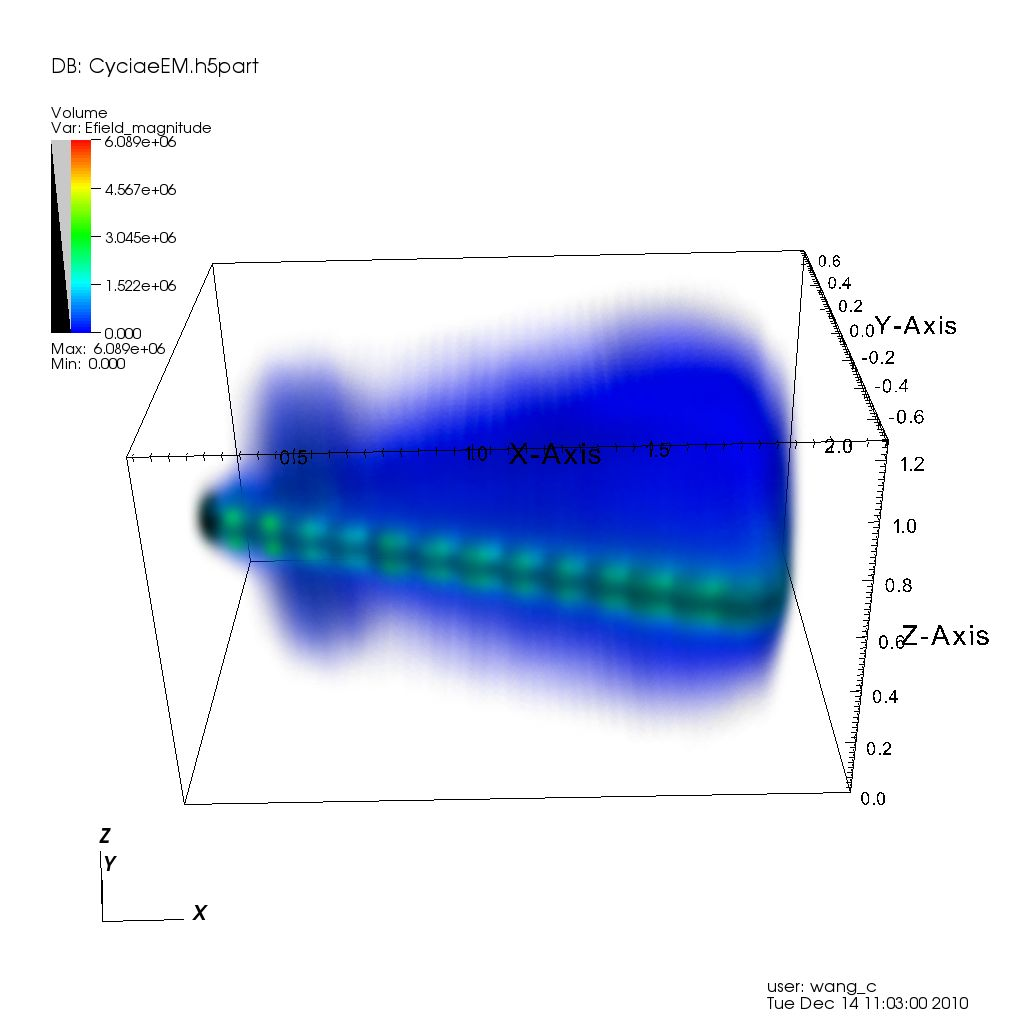
\includegraphics[width=1\textwidth]{visit0001.jpeg}
\end{center}
\caption{Electric field part in FM3DH5Block\_nonescale type field map.\label{fig:eme}}
\end{figure}

\begin{figure}[H]
\begin{center}
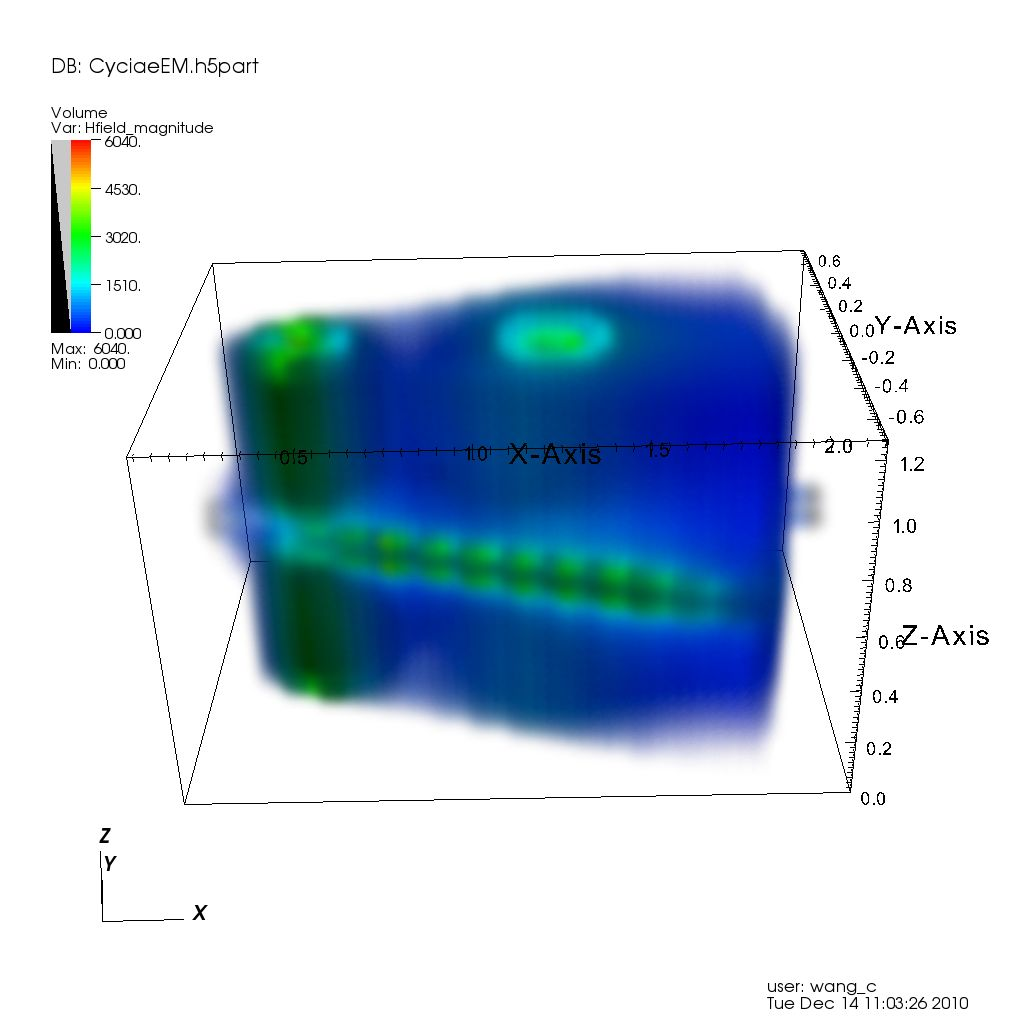
\includegraphics[width=1\textwidth]{visit0002.jpeg}
\end{center}
\caption{Magnetic field part in FM3DH5Block\_nonescale type field map.\label{fig:emm}}
\end{figure}

\begin{figure}[H]
\begin{center}
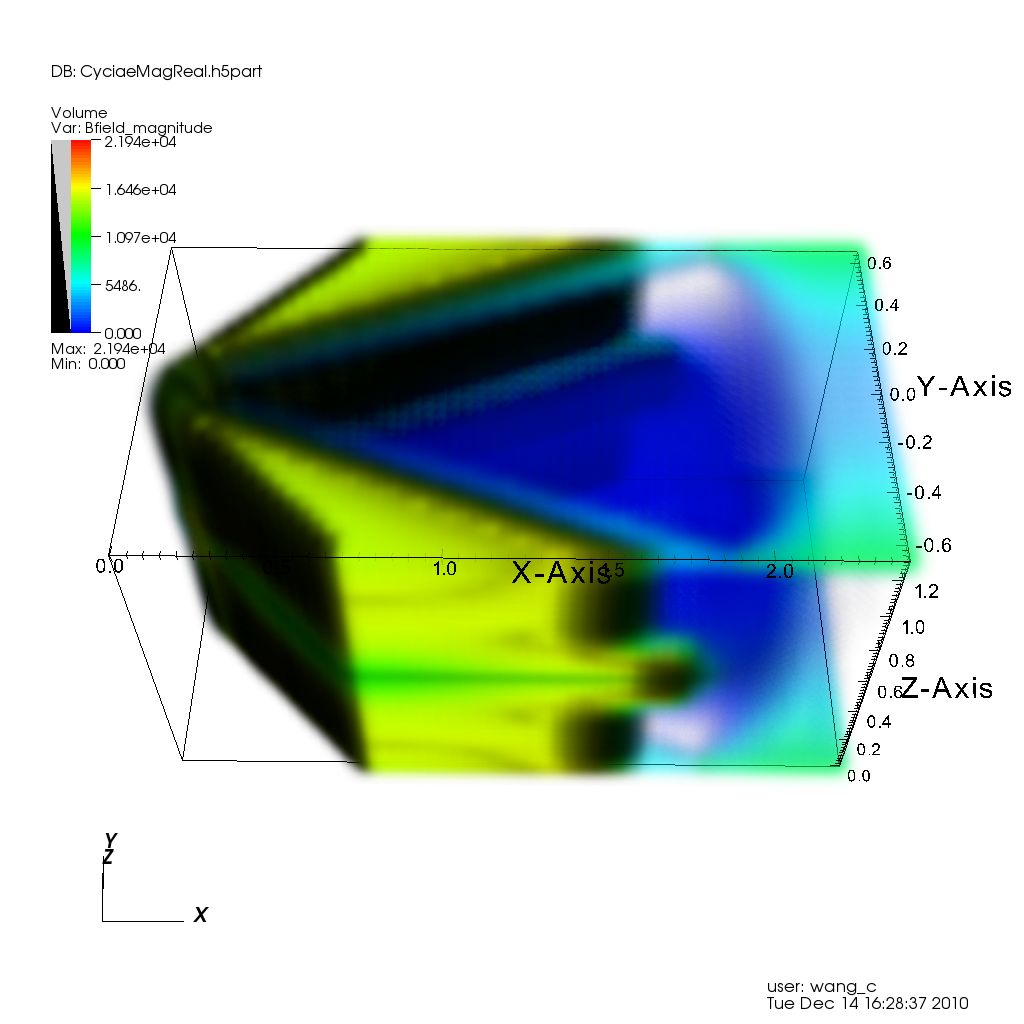
\includegraphics[width=1\textwidth]{visit_Real_mag.jpeg}
\end{center}
\caption{Magnetic flux density in FM3DMagnetoStaticH5Block type field map.\label{fig:mgm}}
\end{figure}

\end{appendices}     
\begin{thebibliography}{99}
\bibitem{SE} M. A. Furman and M. T. F. Pivi,  
Phys. Rev. ST Accel. Beams 5, 124404 (2002)
\bibitem{VH} J. Rodney M. Vaughan, IEEE Transactions on Electron Devices. Vol. 36, No. 9, September 1989
\bibitem{FE} C. Vicente, M. Mattes, D. Wolk, H. L. Hartnagel, J. R. Mosig, D. Raboso, Proc. MULCOPIM 2005, ESTEC-ESA, Noordwijk, The Netherlands, 2005, pp. 11-17
\bibitem{OP} A. Adelmann and Ch. Kraus and Y. Ineichen and  J. Yang,
The \opal\ (Object Oriented Parallel Accelerator Library) 
              Framework, Paul Scherrer Institute, PSI-PR-08-02, 2008
\bibitem{PP} A. Kryazhev, M. Buyanova, V. Semenov, D. Anderson and M. Lisak, J. Puech, L. Lapierre, and J. Sombrin,
Phys. Plasmas, Vol. 9, No. 11, November 2002
\bibitem{PN} R. Udiljak, D. Anderson, and M. Lisak, V. E. Semenov, J. Puech, Phys. Plasmas 14, 033508 2007
\bibitem{NS} S. Anza, C. Vicente, J. Gil, V. E. Boria, B. Gimeno, and D. Raboso, Phys. Plasmas 17, 062110 2010
\bibitem{ST} N. K. Vdovicheva, A. G. Sazontov, and V. E. Semenov, Radiophys. Quantum Electron. 47, 580 2004.

\end{thebibliography} 
\end{document}


% LocalWords:  Anylitical
